\documentclass[
../../EiKI_Summary.tex,
]
{subfiles}
    
\externaldocument[ext:]{../../EiKI_Summary.tex}
% Set Graphics Path, so pictures load correctly
\graphicspath{{../../}}

\begin{document}
\section{Local and Adversarial Search}
(Un-)Informed Search shows some limitations. Typically these algorithms can only handle search spaces with up to $10^{100}$ states due to memory constraints. They also only consider ''paths'' as a solution.

\subsection{Optimization Problems}
\begin{defbox*}
    An optimization problem is a problem where every state can be a solution (to different degrees) but the target is to find the state that optimizes (min, max,\dots) the solution according to an objective function. 

    This means that there is no explicit goal state and also no path to reach it (no cost).

    For example: Darwinian evolution could be seen as an optimization problem.
\end{defbox*}

\begin{defbox}
    [Objective (Evaluation) Function]
    An objective function shows how good a state is, also in comparision to other states. Its value is minimized or maximized depending on the problem.
\end{defbox}

\subsubsection{Terminology}
\begin{defbox}
    [Convergence]
    Describes a sequence of (function) values that approach a limit / value more and more.
\end{defbox}

\begin{minipage}
    [t]{0.5\textwidth}
    \begin{defbox}
        [Global Optimum]
        The \defc{extremum} of an objective function over the \textbf{entire} input search space
    \end{defbox}
\end{minipage}
\begin{minipage}
    [t]{0.5\textwidth}
    \begin{defbox}
        [Local Optimum]
        The \defc{extremum} of an objective function over \textbf{a subset} of the input search space
    \end{defbox}
\end{minipage}

\begin{figure}[H]
    \centering
    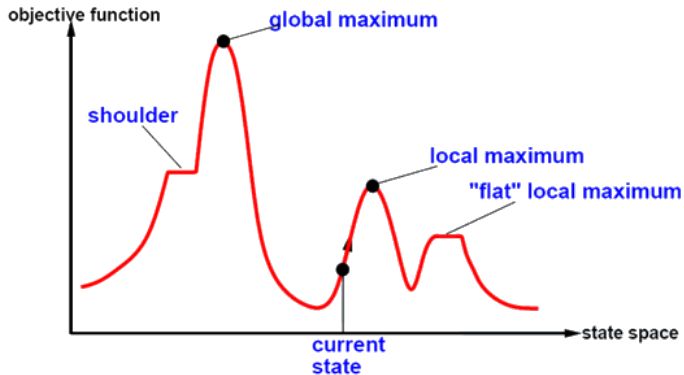
\includegraphics[width=0.6\textwidth]{Pics/04/GlobalLocalOptimum.png}
\end{figure}

\newpage

\subsection{Local Search}
\begin{defbox*}
    Local Search algorithms traver only a single state rather than saving multiple paths. It modifies its state iterative, trying to improve a specific criteria.
\end{defbox*}

Optimization problems often times do not care about the path taken, but only to fulfill the goal constraint.

\begin{minipage}
    [t]{0.5\textwidth}
    \begin{defbox}
        [Advantages]
        \begin{itemize}
            \item Uses little and constant memory
            \item Finds reasonable solution is large state spaces
        \end{itemize}
    \end{defbox}
\end{minipage}
\begin{minipage}
    [t]{0.5\textwidth}
    \begin{defbox}
        [Disadvantages]
        \begin{itemize}
            \item No guarantee for completeness or optimality
        \end{itemize}
    \end{defbox}
\end{minipage}

Basic Idea (Travelling Salesman Problem):
\begin{itemize}
    \item Start with a complete but likely suboptimal tour
    \item Modify the tour (e.g. pairwise swap) to improve the objective function
    \item Repeat until the tour is sufficiently good
    \item This approach often gets very good results quickly
\end{itemize}

\subsubsection{Hill Climbing}

\textbf{Basic Idea:}
\begin{itemize}
    \item Expand the current state
    \item Move to the one with the highest value
    \item Repeat until a maximum is reached
\end{itemize}

\begin{codebox}
    [Hill Climbing]
    \begin{algorithm}[H]
        \SetKwFunction{hillclimb}{hill\_climbing}
        \SetKwFunction{makenode}{make\_node}
        \SetKwFunction{inist}{initial\_state}
        \SetKwFunction{hivasu}{highest\_valued\_successor}
        \SetKwFunction{valued}{value}
        \SetKwFunction{state}{state}
        
        \Fn{\hillclimb{problem}}{
            current = \makenode{\inist{problem}}\;
            neighbor\;
            \While{true}{
                neighbor = \hivasu{current}\;
                \If{\valued{neighbor} $\leq$ \valued{current}}{
                    \KwRet \state{current}\;
                }
                current = neighbor\;
            }
        }
    \end{algorithm}
\end{codebox}
            
\begin{minipage}
    [centering]{0.6\textwidth}
    \textbf{Ridge Problem:}\\
    Most Local Search algorithms are implemented by expanding their neighbors and then selecting the one that increases the objective function the most. Often times the problem space is not as simple as that theres only two neighbors, resulting in a more ''3D'' or higher search space. This can cause an issue, when all neighbors are worse than the current state, but the seach space has an uphill. 
\end{minipage}
\begin{minipage}
    [c]{0.4\textwidth}
    \centering
    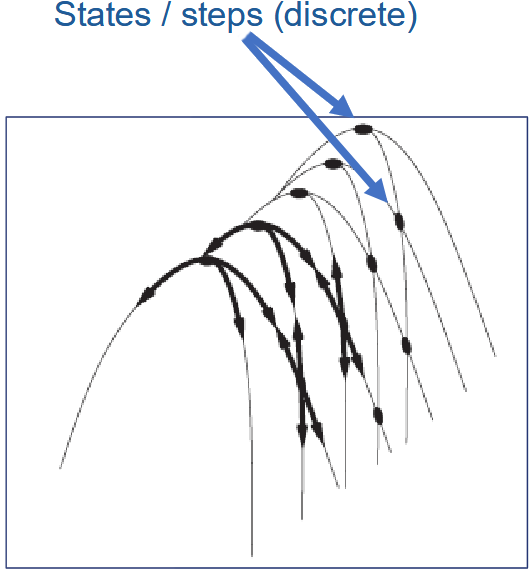
\includegraphics[width=0.75\textwidth]{Pics/04/RidgeProblem.png}
\end{minipage}

\textbf{Problem - Local Optima:}
\begin{itemize}
    \item Algorithm will stop at the nearest local optima
    \item This might be very far from the global optimum (plateus, ridges, shoulders\dots)
    \item Solution: Random Restart
    \begin{itemize}
        \item Random initial positions result in different local optima
        \item $\rightarrow$ Iterate over multiple local optima and select the best one
    \end{itemize}
    \item Alternative Solution: Stochastic Hill Climbing
    \begin{itemize}
        \item Select successor randomly with a higher chance for better successors
    \end{itemize}
\end{itemize}

\subsubsection{Gradient Descent}
As mentioned before, search spaces often are not only 2-dimensional, as we might need to consider multiple features. This, of course, makes it much harder to find an optimal solution with higher dimensional search spaces.

\begin{figure}
    [H]
    \centering
    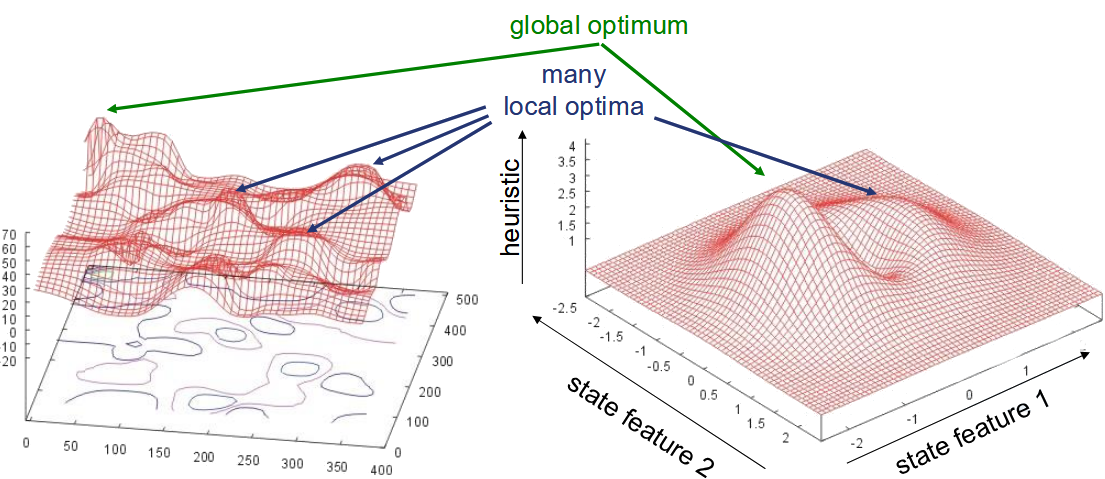
\includegraphics[width=0.8\textwidth]{Pics/04/MultiDimensionalSearchSpace.png}
\end{figure}

Before our objective function only had a single input feature, now we also have to consider more.

\begin{minipage}
    [t]{0.5\textwidth}
    \begin{defbox}
        [Gradient]
        The \defc{derivative} of a function that has more than one input variable. In mathematics it would be known as the \defc{slope} of a function, which measures the change in all weights with regard to the change in error.
    \end{defbox}
\end{minipage}
\begin{minipage}
    [t]{0.5\textwidth}
    \begin{defbox}
        [Gradient Descent]
        The \defc{gradient descent} is an optimization algorithm. It can be considered as Hill-Climbing in continous state space.
    \end{defbox}
\end{minipage}

\begin{defbox}
    [Gradient Descent: Working Principle]
    \begin{minipage}
        [t]{0.5\textwidth}
        \begin{flushright}
            \defc{Gradient Vector} \hspace{10pt}

            \begin{smallmathbox*}
                $\nabla J(\underline{\theta}) = \left[\dfrac{\partial J(\underline{\theta})}{\partial \theta_0}, \dots, \dfrac{\partial J(\underline{\theta})}{\partial \theta_n}\right]$
            \end{smallmathbox*}
        \end{flushright}
    \end{minipage}
    \begin{minipage}
        [t]{0.5\textwidth}
        \begin{flushleft}
            \hspace{10pt}\defc{Cost Function}

            \begin{smallmathbox*}
                $J(x_1, x_2, \dots, x_n)$
            \end{smallmathbox*}
        \end{flushleft}
    \end{minipage}
    \\

    We now want to minimize over the continous variables \inlmathbox{$x_1, x_2, \dots, x_n$}.
    \begin{enumerate}
        \item Compute gradient: \inlmathbox{$\dfrac{\partial}{\partial x_i} J(x_1, x_2, \dots, x_n)\quad \forall i \in n$}
        \item Take a step downhill in the direction of the gradient: \inlmathbox{$x_i\prime = x_i - \lambda \dfrac{\partial}{\partial x_i} J(x_1, x_2, \dots, x_n)$}
        \item If \inlmathbox{$J(x_1\prime, x_2\prime, \dots, x_n\prime) < J(x_1, x_2, \dots, x_n)$}, accept move, else reject.
        \item Repeat until desired accuracy is reached
    \end{enumerate}
    
    \begin{minipage}
        [t]{0.4\textwidth}
        \centering
        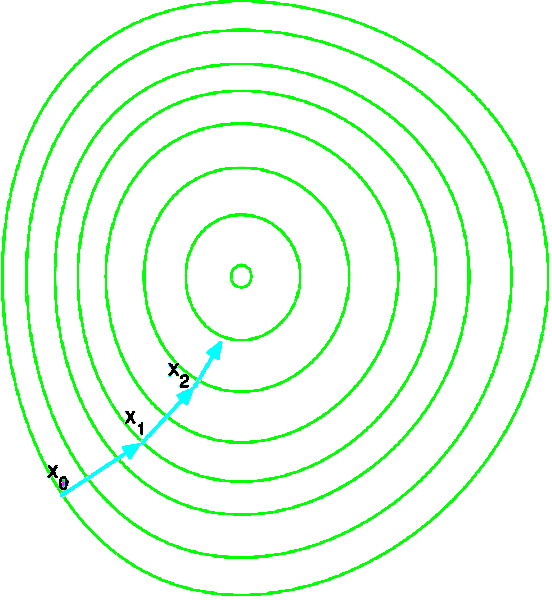
\includegraphics[width=0.9\textwidth]{Pics/04/GradientDescent1.png}
    \end{minipage}
    \begin{minipage}
        [t]{0.6\textwidth}
        \centering
        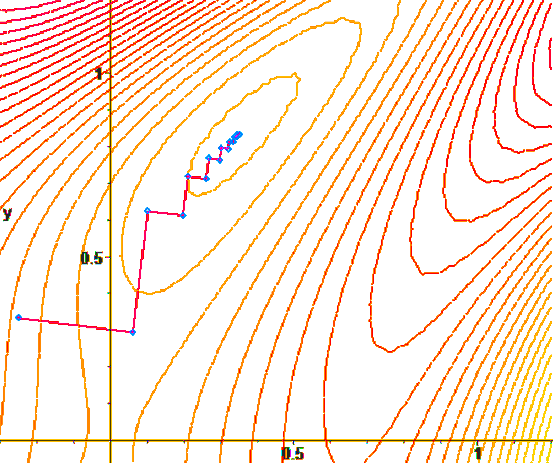
\includegraphics[width=0.75\textwidth]{Pics/04/GradientDescent2.png}
    \end{minipage}
\end{defbox}

\begin{defbox}
    [Learning Rate]
    ''The size of the step taken in the gradient descent''. The \defc{learning rate} is a hyperparameter, controlling how quickly the model adapts to the problem.
\end{defbox}

Finding the right learning rate is a very important task. It can be done by trial and error, or by using a learning rate scheduler.

In general:
\begin{itemize}
    \item \textbf{Smaller learning rate:}
    \begin{itemize}
        \item Smaller changes $\rightarrow$ requires more training epochs
    \end{itemize}
    \item \textbf{Larger learning rate:}
    \begin{itemize}
        \item Larger changes $\rightarrow$ requires fewer training epochs
        \item Can converge to local optima or not at all
    \end{itemize}
\end{itemize}

Determining the gradient can be difficult.
\begin{itemize}
    \item Derive formula using multivariate calculus
    \item Ask mathematician or domain expert
    \item Literature search
    \item Automatic differentiation
\end{itemize}

Gradient Descent in general works well for ''smooth'' spaces; poorly for ''rough'' spaces.

\subsubsection{Beam Search}
\textbf{Basic Idea:}
\begin{itemize}
    \item Keep track of k states (beam size) rather than just one
\end{itemize}
\begin{enumerate}
    \item Start with k randomly generated states
    \item At each iteration, all successors of all k states are generated
    \item Select the k best successors from complete list
    \item Repeat
\end{enumerate}

\begin{figure}
    [H]    
    \begin{minipage}
        [t]{0.5\textwidth}
        \centering
        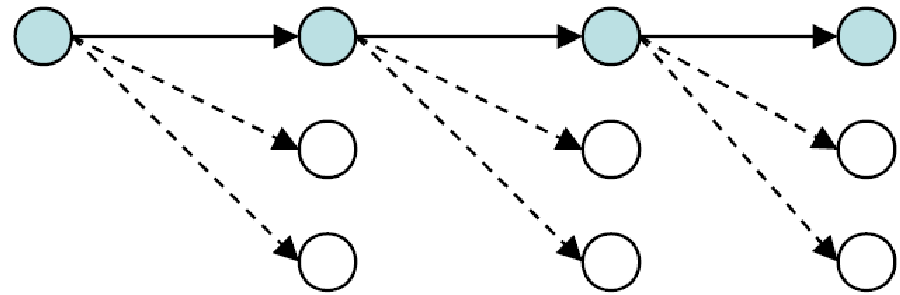
\includegraphics[valign=T,width=0.9\textwidth]{Pics/04/BeamSearchHillClimb.png}
    \end{minipage}
    \begin{minipage}
        [t]{0.5\textwidth}
        \centering
        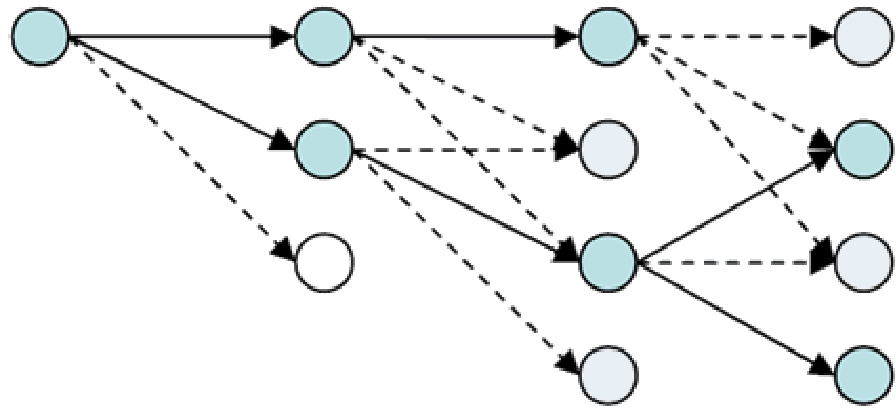
\includegraphics[valign=T,width=0.9\textwidth]{Pics/04/BeamSearch.png}
    \end{minipage}
\end{figure}

\subsubsection{Simulated Annealing}
\textbf{Basic Idea:}
\begin{itemize}
    \item Use hill-climbing, but occasionally take a step into a direction that does not show improvement
    \item Reduce the probability of a down-hill step and decrease the size of the step as the number of iterations grows
    \item Allows some ''bad moves'' to escape local optima
\end{itemize}

\begin{codebox}
    [Simulated Annealing Algorithm]
    \begin{algorithm}[H]
        \SetKwFunction{simann}{simulated\_annealing}
        \SetKwFunction{makenode}{make\_node}
        \SetKwFunction{inist}{initial\_state}
        \SetKwFunction{selransuc}{select\_random\_successor}
        \SetKwFunction{valued}{value}
        \SetKwFunction{rando}{random\_number}

        \tcp{schedule maps time t to temperature T}
        \Fn{\simann{problem, schedule}}{
            current = \makenode{\inist{problem}}\;
            temperature\;
            next\;
            \For{t = 1 to $\infty$}{
                temperature = schedule[t]\;
                next = \selransuc{current}\;
                $\Delta E$ = \valued{next} - \valued{current}\;
                \If{$\Delta E > 0$}{
                    current = next\;
                }
                \tcp{Still accepts worse solution with a probability of $e^{\Delta E/\text{temperature}}$}
                \ElseIf{\rando{0,1} $<$ $e^{\Delta E/\text{temperature}}$}{
                    current = next
                }   
            }
        }
    \end{algorithm}
\end{codebox}

\begin{defbox}
    [Temperature]
    \begin{minipage}
        [c]{0.6\textwidth}
        Temperature is a hyperparameter, controlling how frequently we accept worse solutions to escape local optima. Temperature usually decays exponentially.
    \end{minipage}
    \begin{minipage}
        [c]{0.4\textwidth}
        \centering
        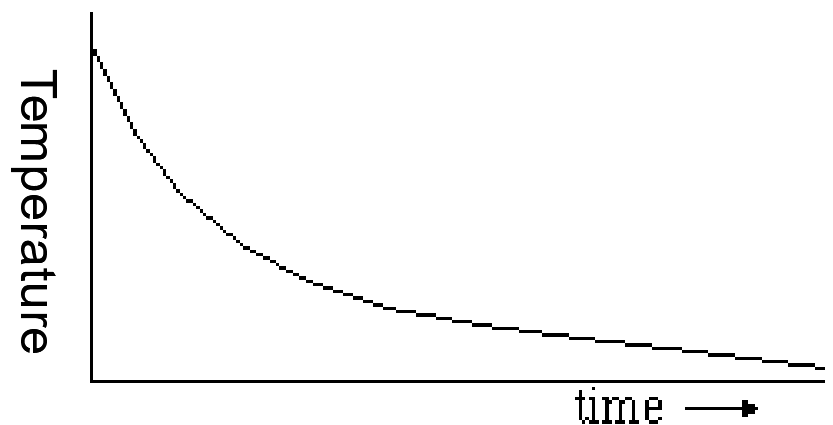
\includegraphics[valign=T,width=0.75\textwidth]{Pics/04/TemperatureOverTime.png}
    \end{minipage}
\end{defbox}

Simulated Annealing converges to a global optimum \textbf{if} the temperature is lowered slowly enough. This is not a strong claim as even random guessing would eventually yield the global optimum. 

As such, simulated annealing can take a very long time.

\subsection{Adversarial Search}
\begin{defbox*}
    Adversarial Search assumes an ''adversary'', who acts against the agent. The goal of adversarial search is to plan ahead, while taking the adversarys actions into account.
\end{defbox*}

Adversarial search is often used to model games as search problems. Each player has to consider other players actions and their effect on the game state.

Adversarial search is often time constrained, so it is unlikely to find an optimal solution.

\subsubsection{Games}
\begin{defbox}
    [Zero-Sum Game]
    Describes a game whereby, if one party loses, the other must win, therefore the net change in ''points'' is zero.
\end{defbox}

A game can be defined as a search problem:
\begin{enumerate}
    \item \defc{\texttt{Initial State}:} Game set-up
    \item \defc{\texttt{Player(s)}:} Specifies which players turn it is
    \item \defc{\texttt{Action(s)}:} Returns all possible moves in state s
    \item \defc{\texttt{Result(s, a)}:} Specifies the state s$\prime$ after action a in state s is taken
    \item \defc{\texttt{Terminal(s)}:} Tests if state s fulfills the goal/terminal constraints
    \item \defc{\texttt{Utility(s, p)}:} Returns a numeric value for a terminal state s from the perspective of player p
\end{enumerate}

\begin{defbox}
    [Game Trees]
    Game Trees are used to represent the possible states of a game. Hereby each level corresponds to a player. The \defc{root node} is always the initial (empty) state with current player. \defc{Leaf Nodes} are always terminal states. Every \defc{terminal node} has a utility value corrsponding to the outcome of the game (e.g. $+1$ for a win, $0$ for a draw, $-1$ for a loss).

    \begin{center}
        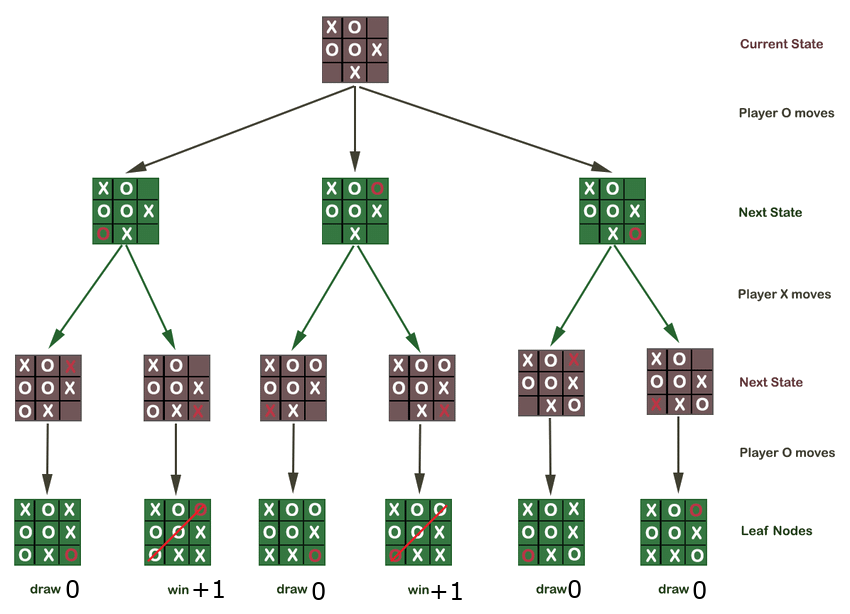
\includegraphics[width=0.6\textwidth]{Pics/04/TicTacToeGameTree.png}
    \end{center}
\end{defbox}

\subsubsection{Games vs. Search Problems}
\begin{itemize}
    \item ''Unpredictable'' opponent
    \begin{itemize}
        \item Specify a move for every possible reply
        \item Different goals for every agent
    \end{itemize}
    \item Time limits
    \begin{itemize}
        \item Likely not enough time to find a goal state
        \item Needs approximation
    \end{itemize}
    \item Most games are
    \begin{itemize}
        \item Deterministic, turn-based, two-player, zero-sum
    \end{itemize}
    \item Real problems are
    \begin{itemize}
        \item Stochastic, parallel, multi-agent, utility based
    \end{itemize}
\end{itemize}

\subsubsection{Minimax Algorithm}
\textbf{Basic Idea:}
\begin{itemize}
    \item Build a game tree where nodes represent the states of the game and edges represent the possible moves.
    \item The players:
    \begin{itemize}
        \item \defc{MIN:} Decreases the chances of \defc{MAX} winning (Opponent)
        \item \defc{MAX:} Increases his own chances of winning (Agent)
    \end{itemize}
    \item Players take alternating turns following their respective strategies.
    \item Choose move to position with the highest \defc{minimax value}
    \item Assume opponent to play the best response to their own action 
\end{itemize}

\begin{codebox}
    [Minimax Algorithm]
    \begin{algorithm}
        [H]
        \SetKwFunction{minimaxdec}{minimax\_decision}
        \SetKwFunction{maxval}{maximizer}
        \SetKwFunction{minval}{minimizer}
        \SetKwFunction{isterminal}{is\_terminal}
        \SetKwFunction{utility}{utility}
        \SetKwFunction{successor}{get\_successors}
        \SetKwFunction{action}{get\_action}
        \SetKwFunction{maxi}{max}
        \SetKwFunction{mini}{min}

        \Fn{\minimaxdec{state}}{
            v = \maxval{state}\;
            \tcp{Returns the action that leads to state with utility value v}
            \KwRet \action{v, \successor{state}}\;
        }
        \Fn{\maxval{state}}{
            \If{\isterminal{state}}{
                \KwRet \utility{state}\;
            }
            v = -\infty\;
            \For{s in \successor{state}}{
                v = \maxi{v, \minval{s}}\;
            }
            \KwRet v\;
        }
        \Fn{\minval{state}}{
            \If{\isterminal{state}}{
                \KwRet \utility{state}\;
            }
            v = \infty\;
            \For{s in \successor{state}}{
                v = \mini{v, \maxval{s}}\;
            }
            \KwRet v\;
        }
    \end{algorithm}
\end{codebox}

\begin{defbox}
    [Characteristics]
    \begin{itemize}
        \item \defc{Optimality}: Yes, assuming an optimal opponent
        \item \defc{Completeness}: Yes, if the tree is finite (e.g. no infinite game loops)
        \item \defc{Time Complexity}: $O(b^m)$
        \item \defc{Space Complexity}: $O(b\cdot m)$
        \item (b is the branching factor, m is the maximum depth)
    \end{itemize}
\end{defbox}

\begin{figure}[H]
    \centering
    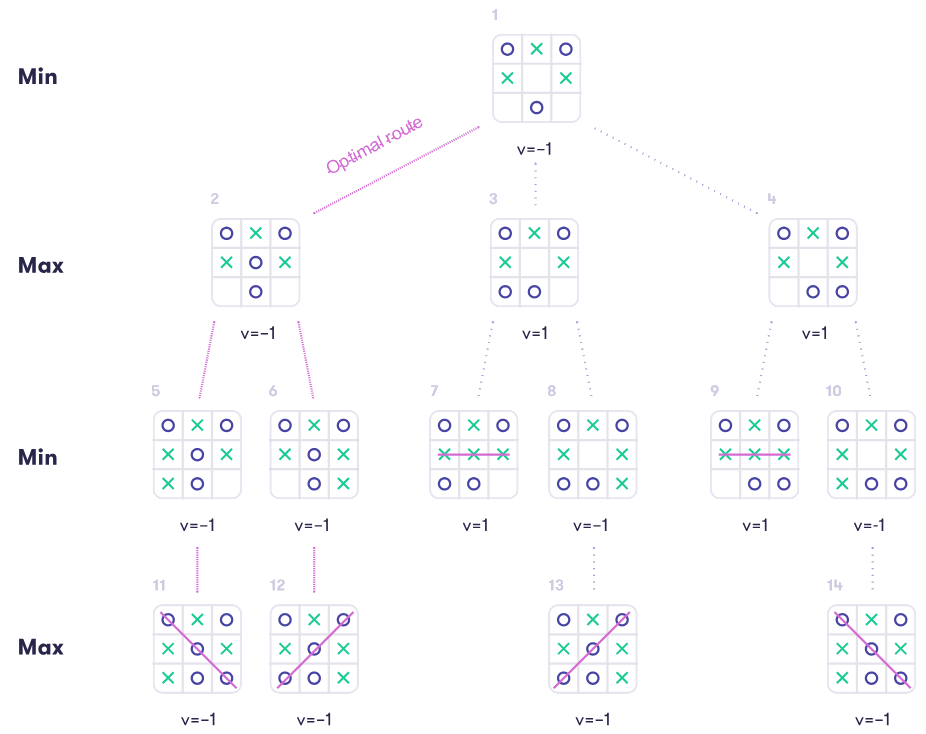
\includegraphics[width=0.7\textwidth]{Pics/04/MinimaxEx.png}
\end{figure}

\textbf{Problem:}\\
Many games have too many possible moves and go on for too long which causes the time complexity to grow exponentially. Go for example has a branching factor of about 250 and can go on for 150+ turns, which would result in approximately $5\times 10^{359} +$ iterations in the worst case. 

\subsubsection{Alpha-Beta Pruning}
\begin{defbox*}
    A modified, optimized version of \defc{Minimax Algorithm}. It uses \defc{pruning} to reduce the amount of exploration without compromising the correctness of minimax.
\end{defbox*}

Alpha-Beta Pruning is based on two parameters
\begin{itemize}
    \item \defc{Alpha:} The best (highest-valued) choice found so far at any point along the path of the Maximizer to the root. Initial Value: $-\infty$
    \item \defc{Beta:} The best (lowest-valued) choice found so far at any point along the path of the Minimizer to the root. Initial Value: $+\infty$ 
\end{itemize}

\textbf{Basic Idea:}\\
Remove all nodes which are not affecting the final decision, but slow down the algorithm.

\begin{codebox}
    [Alpha-Beta Pruning Algorithm]
    \begin{algorithm}[H]
        \SetKwFunction{alphabeta}{alpha\_beta}
        \SetKwFunction{maximizer}{maximizer}
        \SetKwFunction{minimizer}{minimizer}
        \SetKwFunction{successor}{get\_successors}
        \SetKwFunction{minim}{min}
        \SetKwFunction{maxim}{max}
        \SetKwFunction{isterminal}{is\_terminal}
        \SetKwFunction{utility}{utility}

        \Fn{\alphabeta{state}}{
            alpha = -\infty\;
            beta = +\infty\;
            v = \maximizer{state, alpha, beta}\;
            \KwRet v\;
        }
        \Fn{\maximizer{state, alpha, beta}}{
            \If{\isterminal{state}}{
                \KwRet \utility{state}\;
            }
            v = -\infty\;
            \For{s in \successor{state}}{
                eval = \minimizer{s, alpha, beta}\;
                v = \maxim{v, eval}\;
                alpha = \maxim{alpha, v}\;
                \If{beta $\leq$ alpha}{
                    break\;
                }
            }
            \KwRet v\;
        }
        \Fn{\minimizer{state, alpha, beta}}{
            \If{\isterminal{state}}{
                \KwRet \utility{state}\;
            }
            v = +\infty\;
            \For{s in \successor{state}}{
                eval = \maximizer{s, alpha, beta}\;
                v = \minim{v, eval}\;
                beta = \minim{beta, v}\;
                \If{beta $\leq$ alpha}{
                    break\;
                }
            }
            \KwRet v\;
        }
    \end{algorithm}
\end{codebox}

\newpage
\textbf{Differences to Minimax:}
\begin{itemize}
    \item Max Player will only update alpha
    \item Min Player will only update beta
    \item While backtracking, the node values will be passed to upper nodes instead of alpha and beta
    \item Alpha and beta will only be passed to child nodes
\end{itemize}

\textbf{Problems:}
\begin{itemize}
    \item Needs a fast evaluation function
    \item Games with large branching factors (e.g. Go) exploration with alpha-beta pruning is very slow
\end{itemize}
\end{document}